%
% $Id: paper.tex,v 1.4 2005/04/04 10:38:07 kiniry Exp $
%

\documentclass{entcs}

% \usepackage{latex8}
\usepackage{times}
\usepackage{ifpdf}
% \usepackage{a4wide}

\ifpdf
\usepackage[pdftex]{graphicx}
\else
\usepackage{graphicx}
\fi

% \usepackage{html}
% \usepackage{url}
\usepackage{xspace}
%\usepackage{doublespace}
\usepackage{tabularx}
\usepackage{epsfig}
% \usepackage{amsmath}
% \usepackage{amsfonts}
% \usepackage{amssymb}
% \usepackage{eucal}
% \ifpdf
% \usepackage[centredisplay]{diagrams}
% \else
% \usepackage[centredisplay,PostScript=dvips]{diagrams}
% \fi
\usepackage{float}

% \ifpdf
% \usepackage[pdftex,bookmarks=false,a4paper=true,
%            plainpages=false,naturalnames=true,
%            colorlinks=true,pdfstartview=FitV,
%            linkcolor=blue,citecolor=blue,urlcolor=blue,
%            pdfauthor="Joseph R. Kiniry"]{hyperref}
% \else
% \usepackage[dvips,linkcolor=blue,citecolor=blue,urlcolor=blue]{hyperref}
% \fi

\newcommand{\todo}{\textbf{TODO: }}
\newcommand{\sstt}{\begin{small}\begin{alltt}}
\newcommand{\estt}{\end{alltt}\end{small}}
\newcommand{\TODO}{\Large\textbf{TODO }\normalsize}
\newcommand{\tablesize}{\footnotesize}
\newcommand{\cf}{cf.,\xspace}
\newcommand{\eg}{e.g.,\xspace}
\newcommand{\ie}{i.e.,\xspace}
\newcommand{\etc}{etc.\xspace}
\newcommand{\myhref}[2]{\ifpdf\href{#1}{#2}\else\htmladdnormallinkfoot{#2}{#1}\fi}
% \newcommand{\myhref}[2]{\emph{#2}}

%---------------------------------------------------------------------
% New commands, macros, etc.
%---------------------------------------------------------------------

%% \input{kt}

%=====================================================================

\begin{document}

\begin{frontmatter}

\title{A Lightweight Theorem Prover Interface for Eclipse}

\author{Julien Charles\thanksref{charles}}

\address{Everest Group\\
  INRIA Sophia Antipolis\\
  2004 Route des Lucioles - BP 93\\
  FR-06902 Sophia Antipolis, France}

\author{Joseph R.~Kiniry\thanksref{kiniry}}

\address{Systems Research Group\\
  School of Computer Science and Informatics\\
  University College Dublin\\
  Belfield, Dublin 4, Ireland}

\thanks[charles]{Email:\href{mailto:julien.charles@sophia.inria.fr}
  {\texttt{\normalshape julien.charles@sophia.inria.fr}}}
\thanks[kiniry]{Email:\href{mailto:joseph.kiniry@ucd.ie}
  {\texttt{\normalshape joseph.kiniry@ucd.ie}}}

\maketitle

%======================================================================
\thispagestyle{empty}
\begin{abstract}

  An abstract.  

\end{abstract}

\end{frontmatter}

%=====================================================================
\section{Introduction}

An introduction.

%=====================================================================
\section{User Interfaces for Theorem Proving}

%~~~~~~~~~~~~~~~~~~~~~~~~~~~~~~~~~~~~~~~~~~~~~~~~~~~~~~~~~~~~~~~~~~~~~
\subsection{Command-line Interfaces}
All the provers we are targeting (Coq, PVS, Isabelle), have command line interfaces as 
some top-level. These top-level are all alike. It allows to send some commands
to the prover and receive its answers. Usually the standard output is
used for the dialog and the error ouput used to show the prompt.

One of the typical interaction with a top-level can be to have an open text file
where one can stock all the command steps involved and cut and paste its 
content to the top-level and await its results. This user-active kind of 
interaction is somewhat unnatural. That's why usually these basic interactions
are wrapped up in a graphical environment like in Emacs or for Coq
in its own IDE Coqide.



%~~~~~~~~~~~~~~~~~~~~~~~~~~~~~~~~~~~~~~~~~~~~~~~~~~~~~~~~~~~~~~~~~~~~~
\subsection{Emacs}
\todo{jrk, I think you are much more qualified than me for the Emacs part}
\subsubsection{PVS }
\subsubsection{PG}
%~~~~~~~~~~~~~~~~~~~~~~~~~~~~~~~~~~~~~~~~~~~~~~~~~~~~~~~~~~~~~~~~~~~~~
\subsection{Eclipse}
The Eclipse main project can be used like emacs, as a front-end 
for an integrated development environment, or more generally as
a Rich Client Platform \cite{eclipse-rcp}. 
%~~~~~~~~~~~~~~~~~~~~~~~~~~~~~~~~~~~~~~~~~~~~~~~~~~~~~~~~~~~~~~~~~~~~~
\subsubsection{Proof General Toolkit}
\todo{I see more or less things to write for PGToolkit... but I'm not quite
sure what to put in what follows...}\\
Motivations - IDE and IVE integration

Requirements - maintain and extend current interface modality

Context of Work - Mobius

%=====================================================================
\section{Design}

\subsection{plugin architecture}
The main architecture is based on an Eclipse plugin hosting several other
plugins. Eclipse, itself is plugin based. This modularity is useful to 
combine its subversion facilities together with CVS to checkout some 
CVS or/and SVN projects made in Coq. Eclipse also permits to manage 
Java programs together with prover interactions really 
if doing some formal program verification.

The interest of this plugin architecture lies also in the extension points 
 in Eclipse. It easily allows to adapt some of the modern 
IDE features to use with the provers a thing which was not the case
with the extensions for Emacs, which are in a way less restrictive
since .
\subsubsection{Plugins in Eclipse}
In Eclipse the plugin architecture is based upon extension point by
extending or providing them. 
Extension points are defined by a unique identifier which is link
to a definition of a XML tag. Programmers wanting to extend
this extension point just have to write an XML file ({\tt plugin.xml}) 
and provide the right parameters to the tag.
The plugin providing the extension point inspects at runtime what was 
specified with the XML tag. One can find the name of a class to load
and afterward instanciate, the name of a resource or a simple String.

Eclipse provides many extension points. Editors for specific files can be
added, binding together a specific icon, an highlighting, the extension of a
file. There are also parts in Eclipse called ViewParts used
\subsubsection{Plugins in plugins in plugins...}
One plugin used from Eclipse is the integrated editor, to edit the 
file for the prover. The main point was using the standard Eclipse file editor
but extending it with some syntax highlight, a way to block some part
of the text (for the prover-already-evaluated part not to be modified). This
way of adding the editor it is integrated within Eclipse the way an Emacs 
file buffer is.  What the editor also provides is an outline a TreeView
used to represent the file in an abstract way. This outline view
is at first nearly empty only containing the file name one is currently
editing. The prover plugins can complete this implementation to give
an outline of the files (in Coq, for instance it gives the type
hierarchy that can be found in a file).

Another plugin is the view part, to show to the user the result of the
interaction with the prover. It is like a log of the user interactions
with the plugin. It needs no input from the user. It is integrated
at the same place as the outline in the Eclipse workspace.

The last extension from Eclipse to be used is the PreferencePage extension.
It handles the preferences needed to be specified for the prover view
like whether to use or not the unicode set of characters.


Right now there are 4 plugins. The base plugin (ProverEditor)
handling all the non-prover specifics interaction. There is a PVS plugin for
PVS interactions, a Coq plugin for the interaction with the Coq proof 
assistant. There is also a plugin to do some higher level interaction 
with the top-level, i.e. provide some high level Java API to control 
a Coq top-level, called the CoqSugar plugin. 
\subsection{ProverEditor}
\todo{Basic description of the functionalities}\\
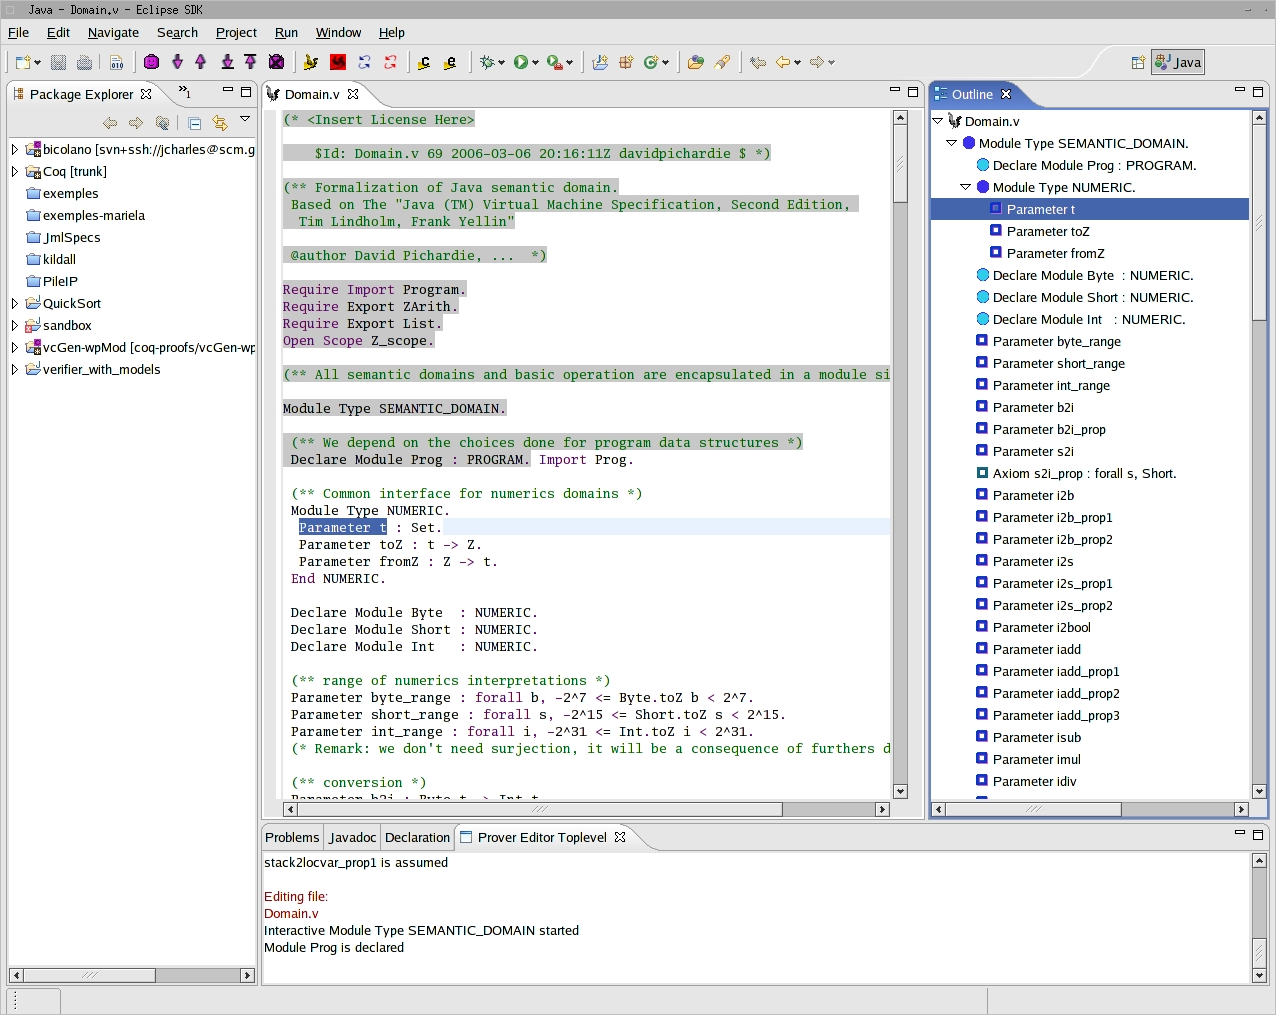
\includegraphics[width=\linewidth]{screenshot1}

A normal execution of ProverEditor...


\includegraphics[width=0.3\linewidth]{toolbar}
the toolbar
\subsubsection{Description}
First we will discuss the main features provided by the ProverEditor plugin
(the basic plugin). This plugin provides some low level handling of the target
prover top-level as well as the basic UI bricks to edit a file from the 
prover and highlight its syntax, show an outline of the file and
progress through a proof with it.

The interaction part gives the ability to manage the interactions like sending
through a stream and receiving data from the top-level from its standard output
and error output.
This part of the plugin correspond to a particular package the 
prover.exec package.
This package evolves mainly around the \\
{\tt prover.exec.toplevel.TopLevel} class
which implements the interface {\tt prover.exec.ITopLevel}. 
When the TopLevel class
is instanciated for a specific prover, it calls a prover specific class giving 
it itself as an argument (passed as an instance from the interface
ITopLevel which has more restrictive methods than the TopLevel class.
The interaction with the top-level is bases on a generic call to sendCommand
if a command has to be sent. In a typical sendCommand scenario, the method
{\tt sendCommand(String)} of the TopLevel class is called, 
afterward a prover specific 
{\tt sendCommand(ITopLevel, String)} is called with an instance of the 
TopLevel as a parameter. The method has to call afterward the primitive
{\tt ITopLevel.sendToProver(String)}, manage the output and throw an 
exception of the type AProverException if something has failed.

There is another method used for the same kind of purpose, the
{\tt undo()} command. It has to trigger an undo command to the
top-level. This method call a prover specific  command
which is meant to undo one step whichever context we are in. In most of
the cases it reduces to a call to the {\tt sendCommand(String)} with the 
right parameter.
For instance for Coq depending on the context it will  reduce to 
sending the {\tt Back 1} command {\tt Undo 1}
 (if we are within a proof) or {\tt Abort}
to cancel a proof.\\


\subsubsection{Extending ProverEditor with provers}
No command line thing 'per se' since
the it is still entirely configured through Eclipse
the package prover.exec anyway it does not use any of the graphical 
Eclipse's API beside the Preference Page
%\subsection{component use via command-line}

\todo{explain properly how to extend}
To add a new prover:\\

First :\\
Create a plugin project within eclipse.\\
Extend the extension point:\\
org.eclipse.ui.editors\\
with the following standard parameters:\\
class="prover.gui.editor.ProverEditor"\\
contributorClass="org.eclipse.ui.editors.text.TextEditorActionContributor"\\
and then customize these ones:\\
extensions=".proof"\\
icon="icons/mypprover.gif"\\
id="myprover.MyProverEditor"\\
name="MyProverEditor"\\

Then:\\
Extend also the extension point\\
prover.editor.prover\\
and fill up all the asked parameters\\
(the extension must be the same as the editor extension)\\
The specified name must be the name you will call the prover afterward.\\
The translator tag need to be specified a class that extends:\\
prover.plugins.AProverTranslator.\\
The toplevel tag need to be specified a class that extends:\\
prover.plugins.IProverTopLevel.\\


%\subsection{component use via Java APIs}


%=====================================================================
\section{Current Plugins}

We have made right now several plugins:
\begin{itemize}
\item the core plugin, containing all the basic features which was described above.
\item the Coq plugin: to handle the interactions with Coq, send parts of a file to Coq
and give an outline of the current edited file.
\item the Coq 'Sugar' plugin, which is used to give a proper API for the Coq top-level.
It is already used in Jack \cite{Jack-Web} (the Java Applet Correctness Kit) an Eclipse plugin
to do static program verification on Java programs annotated with JML.

\item the PVS plugin which is well... finished?
\end{itemize}
\subsection{The Coq plugin}
This plugin is made to do interaction with Coq. The core features
are inside 3 classes. The mandatory plugin class for Eclipse (Eclipse
needs a plugin class in order to consider it has a plugin. This class
is generated automatically by Eclipse. The two other classes are the one
needed to add the extension to ProverEditor: the one used to handle the
top-level and the other one containing mainly the highlighting parts.

There is another part which is less mandatory: the one to handle the outline.
This adds about 10 classes to represents the leafs and nodes of the treeview.
There are 2 kinds of handling: the leaf kind, containing only constructs
like {\tt Definition}, {\tt Parameter} and other single non-imbricated
definitions. There is another kind of construct, the imbricated ones.
In Coq these are the section and the module. These constructs are of
a binary kind, with one to begin them ({\tt Module m.} or {\tt Section s.})
and one to end them ({\tt End m.} or {\tt End s.}).\\
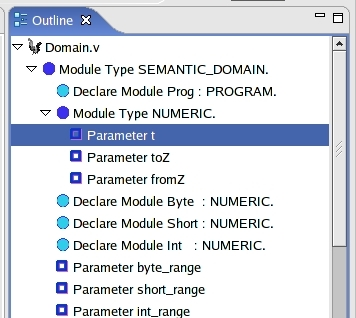
\includegraphics[width=0.5\linewidth]{coqoutline}\\
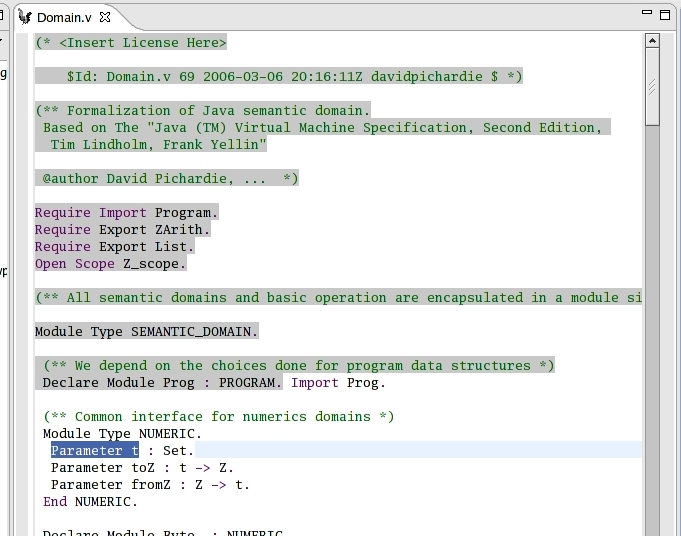
\includegraphics[width=0.6\linewidth]{coqeditor}
\subsection{The Coq sugar-coated plugin}
We have made another plugin which add lots of useless things to the basic plugin,
indeed things that can easily be made over the basic implementation.
The purpose of this plugin is only to ease the use of Coq within ProverEditor.

We have mainly added a more complete API to handle Coq. It has more high-level
'macros'. It subclasses the prover.exec.toplevel.TopLevel to have a real top-level
targeted at Coq. It add some facilities like methods to declare lemmas, do a particular
standard command or parse the output from Coq to give a parsed result of the command
instead of the standard output. For instance, in Coq there is a command {\tt Show Intros} which
is used to know which variable name Coq would use with its  intros command. Here the
method gives an array of String with the different variable names.
In Jack we mainly use this API to pretty print the proof obligations with Coq in order
to have clearer / more user-readable proof obligations.

\subsection{The PVS plugin}
%=====================================================================
\section{Conclusion}

A conclusion.

%~~~~~~~~~~~~~~~~~~~~~~~~~~~~~~~~~~~~~~~~~~~~~~~~~~~~~~~~~~~~~~~~~~~~~
\subsection{Practical Next Steps}

%~~~~~~~~~~~~~~~~~~~~~~~~~~~~~~~~~~~~~~~~~~~~~~~~~~~~~~~~~~~~~~~~~~~~~
\subsection{Graphical Representation of Proof Trees}
Now we use the outline to get an idea of the file structures for Coq and PVS.
We plan to do an enhanced outline that could give a representation
of the proof tree. This structure more akin of the Proof by Pointing.
%~~~~~~~~~~~~~~~~~~~~~~~~~~~~~~~~~~~~~~~~~~~~~~~~~~~~~~~~~~~~~~~~~~~~~
\subsection{Integrating Other Provers}
We plan to include Isabelle/HOL in a near future.
%~~~~~~~~~~~~~~~~~~~~~~~~~~~~~~~~~~~~~~~~~~~~~~~~~~~~~~~~~~~~~~~~~~~~~
\subsection{Open Research Questions and Challenges}


%======================================================================

\bibliographystyle{entcs}
%\bibliography{abbrev,ads,category,complexity,hypertext,icsr,knowledge,languages,linguistics,meta,metrics,misc,modeling,modeltheory,reuse,rewriting,softeng,specification,ssr,technology,theory,web,upcoming,upcoming_conferences,conferences,workshops,verification,escjava,jml,nijmegen}
\bibliography{uitp06}

%======================================================================
% Fin

\end{document}

%%% Local Variables: 
%%% mode: latex
%%% TeX-master: t
%%% End: 
